%\documentclass[10pt,handout]{beamer}
\documentclass[11pt]{beamer}\usepackage[]{graphicx}\usepackage[]{color}
%% maxwidth is the original width if it is less than linewidth
%% otherwise use linewidth (to make sure the graphics do not exceed the margin)
\makeatletter
\def\maxwidth{ %
  \ifdim\Gin@nat@width>\linewidth
    \linewidth
  \else
    \Gin@nat@width
  \fi
}
\makeatother

\definecolor{fgcolor}{rgb}{0.196, 0.196, 0.196}
\newcommand{\hlnum}[1]{\textcolor[rgb]{0.063,0.58,0.627}{#1}}%
\newcommand{\hlstr}[1]{\textcolor[rgb]{0.063,0.58,0.627}{#1}}%
\newcommand{\hlcom}[1]{\textcolor[rgb]{0.588,0.588,0.588}{#1}}%
\newcommand{\hlopt}[1]{\textcolor[rgb]{0.196,0.196,0.196}{#1}}%
\newcommand{\hlstd}[1]{\textcolor[rgb]{0.196,0.196,0.196}{#1}}%
\newcommand{\hlkwa}[1]{\textcolor[rgb]{0.231,0.416,0.784}{#1}}%
\newcommand{\hlkwb}[1]{\textcolor[rgb]{0.627,0,0.314}{#1}}%
\newcommand{\hlkwc}[1]{\textcolor[rgb]{0,0.631,0.314}{#1}}%
\newcommand{\hlkwd}[1]{\textcolor[rgb]{0.78,0.227,0.412}{#1}}%
\let\hlipl\hlkwb

\usepackage{framed}
\makeatletter
\newenvironment{kframe}{%
 \def\at@end@of@kframe{}%
 \ifinner\ifhmode%
  \def\at@end@of@kframe{\end{minipage}}%
  \begin{minipage}{\columnwidth}%
 \fi\fi%
 \def\FrameCommand##1{\hskip\@totalleftmargin \hskip-\fboxsep
 \colorbox{shadecolor}{##1}\hskip-\fboxsep
     % There is no \\@totalrightmargin, so:
     \hskip-\linewidth \hskip-\@totalleftmargin \hskip\columnwidth}%
 \MakeFramed {\advance\hsize-\width
   \@totalleftmargin\z@ \linewidth\hsize
   \@setminipage}}%
 {\par\unskip\endMakeFramed%
 \at@end@of@kframe}
\makeatother

\definecolor{shadecolor}{rgb}{.97, .97, .97}
\definecolor{messagecolor}{rgb}{0, 0, 0}
\definecolor{warningcolor}{rgb}{1, 0, 1}
\definecolor{errorcolor}{rgb}{1, 0, 0}
\newenvironment{knitrout}{}{} % an empty environment to be redefined in TeX

\usepackage{alltt}
%\documentclass[11pt, handout]{beamer}
%\usepackage{handoutWithNotes}
%\usepackage{pgfpages}
\usepackage{etex} % helps fix \newdimen error which is cause when ctable is loaded with other packages
\usepackage{comment}
\usepackage{ctable}
\usepackage{amsmath,amsthm,amssymb}
\newtheorem{rcode}{R code}[section]
\usepackage{url}

%\usepackage[usenames]{xcolor}
\usepackage{color, colortbl}
\usepackage{tikz}
\usepackage[utf8]{inputenc}
\usepackage[T1]{fontenc}
\usepackage{ae}
%\usepackage{aeguill}

\usetikzlibrary{shapes.geometric, arrows,shapes.symbols,decorations.pathreplacing}
\tikzstyle{startstop} = [rectangle, rounded corners, minimum width=3cm, minimum height=1cm, draw=black, fill=pinkish,text width=3.5cm]
\tikzstyle{startstop2} = [rectangle, rounded corners, minimum width=3cm, minimum height=1cm, draw=black, fill=background,text width=2.5cm]
\tikzstyle{startstop3} = [rectangle, rounded corners, minimum width=3cm, minimum height=1cm, draw=black, fill=beige,text width=3.0cm]
\tikzstyle{io} = [trapezium, trapezium left angle=70, trapezium right angle=110, minimum width=2cm, minimum height=1cm, text centered, draw=black, fill=blue!30,text width=1.5cm]
\tikzstyle{process} = [rectangle, minimum width=1cm, minimum height=1cm, text centered, draw=black, fill=orange!30,text width=2cm]
\tikzstyle{decision} = [diamond, minimum width=2cm, minimum height=1cm, text centered, draw=black, fill=green!30]
\tikzstyle{arrow} = [thick,->,>=stealth]
\tikzstyle{both} = [thick,<->,>=stealth, red]

\tikzset{myshade/.style={minimum size=.4cm,shading=radial,inner color=white,outer color={#1!90!gray}}}
\newcommand\mycirc[1][]{\tikz\node[circle,myshade=#1]{};}
\newcommand\myrect[1][]{\tikz\node[rectangle,myshade=#1]{};}
\newcommand\mystar[1][]{\tikz\node[star,star points=15,star point height=2pt,myshade=#1]{};}
\newcommand\mydiamond[1][]{\tikz\node[diamond,myshade=#1]{};}
\newcommand\myellipse[1][]{\tikz\node[ellipse,myshade=#1]{};}
\newcommand\mykite[1][]{\tikz\node[kite,myshade=#1]{};}
\newcommand\mydart[1][]{\tikz\node[dart,myshade=#1]{};}
\newcommand\mycloud[1][]{\tikz\node[cloud,myshade=#1]{};}

%\usepackage{subcaption}
\usepackage{subfig}
%\usepackage{caption}

\mode<presentation>
\usetheme{Hannover}
\usecolortheme{rose}
\setbeamertemplate{navigation symbols}{}
\setbeamertemplate{footline}[frame number]
\setbeamertemplate{caption}[numbered]
\setbeamertemplate{frametitle}[default][left]

\usepackage[]{hyperref}
\hypersetup{
    unicode=false,          
    pdftoolbar=true,        
    pdfmenubar=true,        
    pdffitwindow=false,     % window fit to page when opened
    pdfstartview={FitH},    % fits the width of the page to the window
    pdftitle={atelier R GERAD},    % title
    pdfauthor={Sahir Rai Bhatnagar},     % author
    pdfsubject={Subject},   % subject of the document
    pdfcreator={Sahir Rai Bhatnagar},   % creator of the document
    pdfproducer={Sahir Rai Bhatnagar}, % producer of the document
    pdfkeywords={}, % list of keywords
    pdfnewwindow=true,      % links in new window
    colorlinks=true,       % false: boxed links; true: colored links
    linkcolor=red,          % color of internal links (change box color with linkbordercolor)
    citecolor=blue,        % color of links to bibliography
    filecolor=black,      % color of file links
    urlcolor=cyan           % color of external links
}

%\RequirePackage{color}

% define a bunch of colors
\definecolor{gray}{RGB}{110,110,110}
\definecolor{darkgray}{RGB}{100,100,100}
\definecolor{lightgray}{RGB}{200,200,200}
\definecolor{turquoise}{RGB}{81,193,188}
\definecolor{tomato}{RGB}{255,136,136}
\definecolor{mandarina}{RGB}{229,169,25}
\definecolor{foreground}{RGB}{81,141,193}
\definecolor{background}{RGB}{246,244,240}
\definecolor{highlight}{RGB}{229,169,25}
\definecolor{lowlight}{RGB}{200,200,200}
\definecolor{beige}{RGB}{255,255,240}
\definecolor{pinkish}{RGB}{255,223,247}
%\definecolor{aliceblue}{rgb}{0.94, 0.97, 1.0}
%\definecolor{antiflashwhite}{rgb}{0.95, 0.95, 0.96}

% some convenient commands
\newcommand{\code}[1]{\texttt{#1}}
\newcommand{\high}[1]{\textcolor{highlight}{#1}}
\newcommand{\low}[1]{\textcolor{lowlight}{#1}}
\newcommand{\highcode}[1]{\textcolor{highlight}{\texttt{#1}}}

\setbeamercolor{block body}{bg=beige}
\setbeamertemplate{theorems}[numbered] % so that you can number the R code theorem environments

%\setbeamercovered{highly dynamic}

\newcounter{saveenumi}
\newcommand{\seti}{\setcounter{saveenumi}{\value{enumi}}}
\newcommand{\conti}{\setcounter{enumi}{\value{saveenumi}}}


%\setbeamercolor{subtitle}{fg=turquoise}

%\pgfpagesuselayout{4 on 1}[a4paper, landscape, border shrink=5mm]
%\pgfpagesuselayout{2 on 1 with notes landscape}[a4paper, border shrink=5mm]
\IfFileExists{upquote.sty}{\usepackage{upquote}}{}
\begin{document}






\title[Atelier sur le logiciel R]{Atelier sur le logiciel R}
\subtitle{Un introduction \`{a} la programmation en R}

\author[]{Sahir Rai Bhatnagar%
\thanks{\href{https://github.com/sahirbhatnagar/atelier-R-GERAD}{https://github.com/sahirbhatnagar/atelier-R-GERAD}%
}}

\date{29 juillet 2015}

%\makebeamertitle

\maketitle

\begin{frame}{Programmation de la journée}
\begin{itemize}
\item 09H00 : Début de l'atelier
\item 10H00 - 10H20: pause
\item 12H00 - 13H00: lunch
\item 15H00 -  15H20: pause
\item 17H00 : fin de l'atelier
\end{itemize}
\end{frame}



\begin{frame}{Remerciements}
% \hspace*{-1.9cm}\parbox[t]{\textwidth}
%\frametitle{Acknowledgements}
\begin{columns}[c] % The "c" option specifies centered vertical alignment while the "t" option is used for top vertical alignment

\column{.45\textwidth} % Left column and width

\begin{itemize}
%\scriptsize
\item John Chambers
\item Ross Ihaka et Robert Gentleman
\item Greg Voisin
\item Dr. Vahid Partovi Nia
\item Toi
\end{itemize}

\column{.45\textwidth} % Right column and width
\begin{figure}
\includegraphics[width=0.6\columnwidth]{gerad.png}\\[2mm]
\includegraphics[width=0.6\columnwidth]{udem.png}\\[5mm]
\includegraphics[width=0.6\columnwidth]{hec.png}
%\includegraphics[width=0.7\columnwidth]{Logo-LUDMER.jpg}
\end{figure}

\end{columns}
\end{frame}


\begin{frame}{Avis \#1}
\begin{itemize}
\item Ceci est une \textbf{introduction} au langage R
\pause \item On va faire beaucoup d'exercices
\pause \item N'h\'{e}sitez pas \`{a} posez des questions
\end{itemize}
\end{frame}

\begin{frame}{Avis \#2}
\begin{figure}
\includegraphics[width=1.0\columnwidth]{rstudio.png}\\[5mm]
\includegraphics[width=0.2\columnwidth]{rlogo.png}\\[5mm]
%\includegraphics[width=0.2\columnwidth]{LaTeX_logo.png}
\end{figure}

\textit{Je n'ai aucune relation commerciale avec ces logiciels}

\end{frame}

\begin{frame}{Avis \#3}

\begin{itemize}
\item Le mat\'{e}riel pour cet atelier est bas\'{e} sur plusieurs ressources
\item Voir ce lien pour une liste compl\`{e}te de r\'{e}f\'{e}rences: \href{https://github.com/sahirbhatnagar/atelier-R-GERAD}{https://github.com/sahirbhatnagar/atelier-R-GERAD}
\item Je vous sugg\`{e}re les livres de Vincent Goulet et Hadley Wickham
\end{itemize}

\begin{columns}[c] % The "c" option specifies centered vertical alignment while the "t" option is used for top vertical alignment
\column{.45\textwidth} % Left column and width
\begin{figure}
\includegraphics[width=0.8\columnwidth]{goulet.png}
\end{figure}

\column{.45\textwidth} % Right column and width
\begin{figure}
\includegraphics[width=0.6\columnwidth]{had.jpg}
\end{figure}
\end{columns}

\end{frame}


\begin{frame}[plain]{C'est parti}
\hspace*{-1.5cm}\parbox[t]{\textwidth}{
\begin{center}
\includegraphics[scale=0.51]{introR.jpg}
\end{center}
}
\end{frame}


\setbeamercolor{normal text}{fg=black,bg=background}
\begin{frame}[plain]
\hspace*{-1.0cm}\parbox[t]{\textwidth}{
\begin{block}{Après cet atelier vous devriez \^{e}tre capables de}
\begin{itemize}
\item Comprendre, créer et modifier les 4 objets de bases en R (\code{vector, data.frame, matrix, list}) 
\item Utiliser des fonctions de bases
\item Importer un jeux de données à partir d'un fichier externe
\item Créer un graphique 
\end{itemize}
\end{block}
}
\end{frame}


\section{1.Pr\'{e}sentation du langage R}

\setbeamercolor{normal text}{fg=gray,bg=black}
\begin{frame}[plain]
\hspace*{-1.0cm}\parbox[t]{\textwidth}{
 \begin{center}
  \Huge{\textcolor{white}{1. Pr\'{e}sentation du langage R}}
 \end{center}
 }
\end{frame}


\setbeamercolor{normal text}{fg=black,bg=background}
\begin{frame}[plain]
\hspace*{-1.0cm}\parbox[t]{\textwidth}{
\begin{block}{Objectifs du chapitre}
\begin{enumerate}
\item Comprendre les avantages d'apprendre R
\item Conna\^{\i}tre la provenance du R et ses caract\'{e}ristiques
\item D\'{e}marrer une session R et ex\'{e}cuter des commandes simples
\item Cr\'{e}er, modifier et sauvegarder ses propres fichiers de \mbox{script R}
\end{enumerate}
\end{block}
}
\end{frame}



\setbeamercolor{normal text}{fg=gray,bg=white}
\subsection{Pourquoi \^{e}tes-vous l\`{a}?}

\begin{frame}
 \begin{center}
  \Huge{\textcolor{red}{Pourquoi vous \^{e}tes l\`{a}?}}
 \end{center}
\end{frame}


\begin{frame}{Le langage R gagne en popularit\'{e}}

\vspace{0.1in}

\begin{center}
\includegraphics[scale=0.40]{rankings.png}
\end{center}

\vspace{0.2in}

Les meilleurs langages de programmation en 2015 selon \href{http://spectrum.ieee.org/computing/software/the-2015-top-ten-programming-languages}{\mbox{IEEE Spectrum}} \\
\end{frame}


\begin{frame}{Plus de 100 000 questions pos\'{e}es dans les forums}

\includegraphics[scale=0.40]{stack.png}
\newline
\vspace{0.1in}
%\footenotesize{source: http://r4stats.com/articles/popularity/}
\end{frame}




\begin{frame}{Nombre d'emplois}

\begin{center}
\includegraphics[scale=0.47]{jobs.png}
\end{center}

\vspace{0.05in}

r\'{e}f\'{e}rence: \href{http://r4stats.com/articles/popularity/}{http://r4stats.com/articles/popularity/}\\

\end{frame}



\begin{frame}{Utilis\'{e} dans plusieurs domaines}

\begin{center}
\includegraphics[scale=0.31]{citeR.jpg}
\end{center}

\vspace{0.05in}

Publi\'{e} dans \href{http://www.nature.com/news/programming-tools-adventures-with-r-1.16609}{\textit{Nature}}
\end{frame}


\begin{frame}{Analyser vos données}
\begin{itemize}
  \setlength\itemsep{2em}
\item Plusieurs ressources d'outils statistiques
\item Représenter graphiquement des jeux de données multivariables
\item Intégrer votre code R dans des applications web
\item Assurer la reproductivité de vos analyses
\end{itemize}
\end{frame}



\subsection{Bref historique}

\begin{frame}
 \begin{center}
  \Huge{\textcolor{red}{Bref historique}}
 \end{center}
\end{frame}


\begin{frame}{\`{A} l'origine de R fut le S par John M. Chambers}
\begin{center}
\begin{figure}
\includegraphics[scale=0.10]{john.jpg}
\caption{S, un langage pour programmer avec des donn\'{e}es, developp\'{e} chez Bell Laboratories dans les ann\'{e}es 1970 par une \'{e}quipe de chercheurs men\'{e}e par John M. Chambers}
\end{figure}
\end{center}
\end{frame}


\begin{frame}{Cr\'{e}ateurs}
\begin{center}
\begin{figure}
\includegraphics[scale=0.60]{rr.jpg}
\caption{Inspir\'{e}s par le S, Ross Ihaka (gauche) et Robert Gentleman (droite) de l'Universit\'{e} d'Auckland en Nouvelle-Z\'{e}lande ont lanc\'{e} la premi\`{e}re version de R en 1996}
\end{figure}
\end{center}
\end{frame}


\begin{frame}{Logiciel Libre}
\begin{itemize}
  \setlength\itemsep{2em}
\item 1990-2010: le S a principalement \'{e}t\'{e} popularis\'{e} par une mise en oeuvre commerciale nomm\'{e}e S-PLUS
\pause \item Fin des ann\'{e}es 2000: L'utilisation de S-PLUS diminue en faveur du R, surtout dans les milieux acad\'{e}miques
\pause \item 2 raisons qui ont fortement contribu\'{e} \`{a} la perte d'influence de S-PLUS
\begin{enumerate}
\item \normalsize Disponible gratuitement
\pause \item Ouvert aux contributions de tous
\end{enumerate}
\end{itemize}
\end{frame}



\subsection{Caract\'{e}ristiques de R}

\begin{frame}
 \begin{center}
  \Huge{\textcolor{red}{Caract\'{e}ristiques de R}}
 \end{center}
\end{frame}



\begin{frame}{Langage de programmation orientée objet}
\begin{itemize}
  \setlength\itemsep{2em}
\item Cela permet de facilement trouver et ré-utiliser les résultats de tes analyses
\pause \item Une fonction peut compléter plusieurs t\^{a}ches
\end{itemize}
\end{frame}


\begin{frame}{Langage de programmation interpr\'{e}t\'{e}}
\begin{itemize}
  \setlength\itemsep{2em}
\item Langage de programmation interpr\'{e}t\'{e} (versus \code{C}, \code{C++}, \code{JAVA})
\item Plus accessible qu'un langage compilé $\rightarrow$ ce qui permet aux économistes, écologistes, biologistes, statisticiens, épidémiologistes, etc. d'utiliser R  
\pause \item Le programme que l'on lance pour utiliser R est l'interpr\`{e}te
\pause \item Celui-ci prend des commandes en R qu'il ex\'{e}cutera imm\'{e}diatement
\pause \item  Autre exemple: \code{Python}
\end{itemize}
\end{frame}


\begin{frame}{Logiciel libre (\textit{Open Source})}

\begin{itemize}
  \setlength\itemsep{1.5em}
\item D\'{e}veloppement actif pour la cr\'{e}ation de nouveaux outils dans plusieurs domaines  
\begin{itemize}
\item \href{https://cran.r-project.org/web/views/}{https://cran.r-project.org/web/views/}
\end{itemize} 
\item Facilement voir le code des autres avec GitHub 
\begin{itemize}
\item \href{http://www.r-pkg.org/}{http://www.r-pkg.org/}
\end{itemize}
\item Bien documenter avec beaucoup de ressources gratuites disponibles sur l'internet  
\begin{itemize}
\item \href{http://stackoverflow.com/questions/tagged/r}{stackoverflow}
\item \href{http://www.rdocumentation.org/}{http://www.rdocumentation.org/} \item \href{http://www.r-bloggers.com/}{http://www.r-bloggers.com/} 
\item \href{https://twitter.com/search?q=\%23rstats}{twitter} 
\item \href{http://blog.revolutionanalytics.com/local-r-groups.html}{R user groups}
\item \href{https://www.google.ca/}{Google}
\end{itemize}
\end{itemize}

%\begin{center}
%\begin{figure}
%\includegraphics[scale=0.35]{meta.png}
%\caption{\href{http://www.r-pkg.org/}{http://www.r-pkg.org/}}
%\end{figure}
%\end{center}

\end{frame}



\begin{frame}[fragile]{Outil statistique qui optimize l'approche matricielle}

\begin{itemize}
  \setlength\itemsep{2em}
\item Langage bas\'{e} sur la notion de vecteur, ce qui simplifie les calculs math\'{e}matiques (non seulement la computation mais l'écriture aussi)
\pause \item R\'{e}duit consid\'{e}rablement le recours aux structures it\'{e}ratives
(boucles \code{for, while} , etc.)
\end{itemize}
\pause 
\begin{knitrout}
\definecolor{shadecolor}{rgb}{1, 1, 1}\color{fgcolor}\begin{kframe}
\begin{rcode}\label{unnamed-chunk-1}\begin{alltt}
\hlkwd{c}\hlstd{(}\hlnum{1}\hlstd{,}\hlnum{2}\hlstd{,}\hlnum{3}\hlstd{)} \hlopt{+} \hlkwd{c}\hlstd{(}\hlnum{4}\hlstd{,}\hlnum{5}\hlstd{,}\hlnum{6}\hlstd{)}
\end{alltt}
\begin{verbatim}
## [1] 5 7 9
\end{verbatim}
\end{rcode}\end{kframe}
\end{knitrout}

%\begin{center}
%\begin{figure}
%\includegraphics[scale=0.35]{meta.png}
%\caption{\href{http://www.r-pkg.org/}{http://www.r-pkg.org/}}
%\end{figure}
%\end{center}

\end{frame}





\begin{frame}[fragile]{O\`{u} trouver de l'aide pour une fonction}
\begin{itemize}
  \setlength\itemsep{2em}
%\item Pour l'aide g\'{e}n\'{e}ral: \texttt{help.start()} 
%\item Lorsque l'on conna\^{i}t le nom de la commande R: 
%\item \mbox{\texttt{help(nom de la fonction)}} 
\item \mbox{\texttt{?nom\_de\_la\_fonction}}
%\item \`{A} partir des mot-cl\'{e}s: \texttt{??mot cl\'{e}}
%\begin{itemize}
%\item exemple: \code{??regression}
%\end{itemize}
%\item Toutes les commandes fournies par un package: \code{help(package=nom du package)}
%\begin{itemize}
%\item exemple: \code{help(package = datasets)}
%\end{itemize}
%\item F1 sur votre clavier 
\end{itemize}

\pause 
\begin{knitrout}
\definecolor{shadecolor}{rgb}{1, 1, 1}\color{fgcolor}\begin{kframe}
\begin{rcode}\label{unnamed-chunk-2}\begin{alltt}
\hlcom{# l'aide pour la fonction de régression linéaire 'lm'}
\hlopt{?}\hlstd{lm}
\end{alltt}
\end{rcode}\end{kframe}
\end{knitrout}
\end{frame}


\begin{frame}{La rubrique d'aide}
\begin{itemize}
  \setlength\itemsep{2em}
\item \textbf{Usage:} le nom de la fonction, tous ses arguments et les valeurs par défaut
\pause \item \textbf{Value:} le type d'objet retourné par la fonction
\end{itemize}
\end{frame}


%\begin{frame}{Clavier Mac}
%\vspace{0.1in}
%\begin{center}
%\includegraphics[scale=0.40]{mackey.jpg}
%\end{center}
%\end{frame}

%\begin{frame}{Clavier PC}
%\vspace{0.1in}
%\begin{center}
%\includegraphics[scale=0.40]{pckey.jpg}
%\end{center}
%\end{frame}



%\subsection{Bref Historique et description}





\subsection{D\'{e}marrer une session}

\begin{frame}
 \begin{center}
  \Huge{\textcolor{red}{D\'{e}marrer une session}}
 \end{center}
\end{frame}


\begingroup
\makeatletter
\setlength{\hoffset}{-.5\beamer@sidebarwidth}
\makeatother
\begin{frame}[fragile, plain]
\begin{knitrout}
\definecolor{shadecolor}{rgb}{1, 1, 1}\color{fgcolor}\begin{kframe}
\begin{rcode}\label{label}\begin{alltt}
\hlcom{# Démarrer l'interface pour la documentation}
\hlcom{# et naviguer les différentes ressources}
\hlkwd{help.start}\hlstd{()}

\hlcom{# trouver l'aide pour la fonction rnorm}
\hlopt{?}\hlstd{rnorm}

\hlcom{# Connaitre le répertoire de travail}
\hlkwd{getwd}\hlstd{()}
\end{alltt}
\end{rcode}\end{kframe}
\end{knitrout}
\end{frame}

%\begin{frame}[fragile, plain]
%<<rcode=TRUE, eval=FALSE>>=
%@
%\end{frame}




\begin{frame}[fragile, plain]
\begin{knitrout}
\definecolor{shadecolor}{rgb}{1, 1, 1}\color{fgcolor}\begin{kframe}
\begin{rcode}\label{unnamed-chunk-3}\begin{alltt}
\hlcom{# On additionne}
\hlnum{39} \hlopt{+} \hlnum{3}

\hlcom{# On soustrait}
\hlnum{58} \hlopt{-} \hlnum{16}

\hlcom{# On multiplie}
\hlnum{6} \hlopt{*} \hlnum{7}

\hlcom{# Et on peut même diviser}
\hlnum{8} \hlopt{/} \hlnum{3}
\end{alltt}
\end{rcode}\end{kframe}
\end{knitrout}
\end{frame}



\begin{frame}[fragile, plain]
\begin{knitrout}
\definecolor{shadecolor}{rgb}{1, 1, 1}\color{fgcolor}\begin{kframe}
\begin{rcode}\label{unnamed-chunk-4}\begin{alltt}
\hlcom{# Générer deux vecteurs de nombres pseudo-aléatoires}
\hlcom{# issus d’une loi normale centrée réduite.}
\hlstd{x} \hlkwb{<-} \hlkwd{rnorm}\hlstd{(}\hlnum{50}\hlstd{)}
\hlstd{y} \hlkwb{<-} \hlkwd{rnorm}\hlstd{(}\hlnum{50}\hlstd{)}

\hlcom{# Graphique des couples (x, y)}
\hlkwd{plot}\hlstd{(x, y)}

\hlcom{# Graphique d'un histogramme de x}
\hlkwd{hist}\hlstd{(x)}
\end{alltt}
\end{rcode}\end{kframe}
\end{knitrout}
\end{frame}


\begin{frame}[fragile, plain]
\begin{knitrout}
\definecolor{shadecolor}{rgb}{1, 1, 1}\color{fgcolor}\begin{kframe}
\begin{rcode}\label{unnamed-chunk-5}\begin{alltt}
\hlcom{# voir la matière de x}
\hlstd{x}

\hlcom{# voir les objets de votre workspace}
\hlkwd{ls}\hlstd{()}

\hlcom{# supprimer les deux vecteurs x et y}
\hlkwd{rm}\hlstd{(x,y)}

\hlcom{# voir la matière de x}
\hlstd{x}

\hlcom{# voir les objets de votre workspace}
\hlkwd{ls}\hlstd{()}
\end{alltt}
\end{rcode}\end{kframe}
\end{knitrout}
\end{frame}


\begin{frame}[fragile, plain]
\begin{knitrout}
\definecolor{shadecolor}{rgb}{1, 1, 1}\color{fgcolor}\begin{kframe}
\begin{rcode}\label{unnamed-chunk-6}\begin{alltt}
\hlcom{# Générer la suite 1, 2, ..., 20.}
\hlstd{x} \hlkwb{<-} \hlnum{1}\hlopt{:}\hlnum{20}

\hlcom{# créer un autre vecteur en fonction de x}
\hlstd{y} \hlkwb{<-} \hlnum{2}\hlopt{*}\hlstd{x}\hlopt{+}\hlnum{3}

\hlcom{# créer un data frame de deux colonnes et}
\hlcom{# voir sa matière }
\hlstd{dt} \hlkwb{<-} \hlkwd{data.frame}\hlstd{(x, y)}
\hlstd{dt}

\hlcom{# estimer un modèle linéaire et voir les}
\hlcom{# résultats}
\hlstd{fit} \hlkwb{<-} \hlkwd{lm}\hlstd{(y} \hlopt{~} \hlstd{x,} \hlkwc{data} \hlstd{= dt)}
\hlkwd{summary}\hlstd{(fit)}
\end{alltt}
\end{rcode}\end{kframe}
\end{knitrout}
\end{frame}

\endgroup


\begin{comment}
\begin{frame}[fragile, plain]
\begin{knitrout}
\definecolor{shadecolor}{rgb}{1, 1, 1}\color{fgcolor}\begin{kframe}
\begin{rcode}\label{unnamed-chunk-7}\begin{alltt}
\hlcom{# La fonction ’seq’ sert à générer des suites }
\hlcom{# plus générales.}
\hlkwd{seq}\hlstd{(}\hlkwc{from} \hlstd{=} \hlopt{-}\hlnum{5}\hlstd{,} \hlkwc{to} \hlstd{=} \hlnum{10}\hlstd{,} \hlkwc{by} \hlstd{=} \hlnum{3}\hlstd{)}
\hlkwd{seq}\hlstd{(}\hlkwc{from} \hlstd{=} \hlopt{-}\hlnum{5}\hlstd{,} \hlkwc{length} \hlstd{=} \hlnum{10}\hlstd{)}

\hlcom{# La fonction ’rep’ sert à répéter des valeurs.}
\hlkwd{rep}\hlstd{(}\hlnum{1}\hlstd{,} \hlnum{5}\hlstd{)} \hlcom{# répéter 1 cinq fois}
\hlkwd{rep}\hlstd{(}\hlnum{1}\hlopt{:}\hlnum{5}\hlstd{,} \hlnum{5}\hlstd{)} \hlcom{# répéter le vecteur 1,...,5 cinq fois}
\hlkwd{rep}\hlstd{(}\hlnum{1}\hlopt{:}\hlnum{5}\hlstd{,} \hlkwc{each} \hlstd{=} \hlnum{5}\hlstd{)} \hlcom{# répéter chaque élément cinq fois}
\end{alltt}
\end{rcode}\end{kframe}
\end{knitrout}
\end{frame}



\begin{frame}[fragile, plain]
\begin{knitrout}
\definecolor{shadecolor}{rgb}{1, 1, 1}\color{fgcolor}\begin{kframe}
\begin{rcode}\label{unnamed-chunk-8}\begin{alltt}
\hlcom{# Arithmétique vectorielle}
\hlstd{v} \hlkwb{<-} \hlnum{1}\hlopt{:}\hlnum{12}  \hlcom{# initialisation d’un vecteur}
\hlstd{v} \hlopt{+} \hlnum{2} \hlcom{# additionner 2 à chaque élément de v}
\hlstd{v} \hlopt{* -}\hlnum{12}\hlopt{:-}\hlnum{1} \hlcom{# produit élément par élément}
\hlstd{v} \hlopt{+} \hlnum{1}\hlopt{:}\hlnum{3} \hlcom{# le vecteur le plus court est recyclé}

\hlcom{# Vecteur de nombres uniformes sur }
\hlcom{# l’intervalle [1, 10]. Le point-virgule}
\hlcom{# signifie une nouvelle ligne}
\hlstd{v} \hlkwb{<-} \hlkwd{runif}\hlstd{(}\hlnum{12}\hlstd{,} \hlkwc{min} \hlstd{=} \hlnum{1}\hlstd{,} \hlkwc{max} \hlstd{=} \hlnum{10}\hlstd{); v}

\hlcom{# Pour afficher le résultat d’une affectation,}
\hlcom{# placer la commande entre parenthèses.}
\hlstd{( v} \hlkwb{<-} \hlkwd{runif}\hlstd{(}\hlnum{12}\hlstd{,} \hlkwc{min} \hlstd{=} \hlnum{1}\hlstd{,} \hlkwc{max} \hlstd{=} \hlnum{10}\hlstd{) )}
\end{alltt}
\end{rcode}\end{kframe}
\end{knitrout}
\end{frame}




\begin{frame}[fragile, plain]
\begin{knitrout}
\definecolor{shadecolor}{rgb}{1, 1, 1}\color{fgcolor}\begin{kframe}
\begin{rcode}\label{unnamed-chunk-9}\begin{alltt}
\hlcom{# trouver le répertoire où se trouve le}
\hlcom{# jeux de données 'morley', qui est inclu avec}
\hlcom{# l'installation de R}
\hlstd{filepath} \hlkwb{<-} \hlkwd{system.file}\hlstd{(}\hlstr{"data"}\hlstd{,} \hlstr{"morley.tab"}\hlstd{,}
            \hlkwc{package}\hlstd{=}\hlstr{"datasets"}\hlstd{)}

\hlcom{# importer les données dans un objet appeller 'mm'}
\hlstd{mm} \hlkwb{<-} \hlkwd{read.table}\hlstd{(filepath)}

\hlcom{# Graphique }
\hlkwd{plot}\hlstd{(mm}\hlopt{$}\hlstd{Expt, mm}\hlopt{$}\hlstd{Speed,}
\hlkwc{main}\hlstd{=}\hlstr{"Speed of Light Data"}\hlstd{,} \hlkwc{xlab}\hlstd{=}\hlstr{"Experiment No."}\hlstd{)}

\hlcom{# Terminer la session}
\hlkwd{q}\hlstd{()}
\end{alltt}
\end{rcode}\end{kframe}
\end{knitrout}
\end{frame}
\end{comment}




\section{2.Bases du langage R}

\setbeamercolor{normal text}{fg=gray,bg=black}
\begin{frame}[plain]
\hspace*{-1.0cm}\parbox[t]{\textwidth}{
 \begin{center}
  \Huge{\textcolor{white}{2. Bases du langage R}}
 \end{center}
 }
\end{frame}

\setbeamercolor{normal text}{fg=black,bg=background}
\begin{frame}[plain]
\hspace*{-1.0cm}\parbox[t]{\textwidth}{
\begin{block}{Objectifs du chapitre}
\begin{enumerate}
\item Comprendre ce qui est un fonction et comment l'utiliser
\item Identifier les principaux types d'objets dans R: \code{vector, matrix, data frame} et \code{list} 
\item Cr\'{e}er et manipuler ces objets
\item Importer des fichiers \code{.txt} et \code{.csv}
\item Installer un \textit{package}
\end{enumerate}
\end{block}
}
\end{frame}



\setbeamercolor{normal text}{fg=gray,bg=white}


\subsection{Les fonctions}

\begin{frame}
 \begin{center}
  \Huge{\textcolor{red}{Les fonctions}}
 \end{center}
\end{frame}



\begin{frame}{Définition et appel de fonctions}
\begin{itemize}
 \setlength\itemsep{2em}
\item Plutôt que d'écrire plusieurs lignes de codes pour des choses assez simples et répétitives on fait appel à des \textbf{fonctions}
\pause \item Une fonction est caractérisée par deux composantes:
\pause 
\begin{enumerate}
\normalsize
\item son \textbf{nom}: c'est ce nom qui nous permettra d'appeler la fonction
\pause \item une \textbf{liste d'arguments}: ce sont les informations dont la fonction a besoin pour travailler et renvoyer son résultat
\end{enumerate}
\end{itemize}
\end{frame}





\begin{frame}[fragile]{La syntaxe pour appeler une fonction}
\begin{itemize}
 \setlength\itemsep{2em}
\item Il faut écrire son nom suivi de parenthèses
\pause \item Entre ces parenthèses, nous indiquerons les arguments dont la fonction a besoin:
\begin{center}
\code{nom\_de\_la\_fonction(arguments)}
\end{center}
\end{itemize}
\pause 
\begin{knitrout}
\definecolor{shadecolor}{rgb}{1, 1, 1}\color{fgcolor}\begin{kframe}
\begin{rcode}\label{unnamed-chunk-10}\begin{alltt}
\hlcom{# chercher la rubrique d'aide pour racine carrée}
\hlopt{?}\hlstd{sqrt}

\hlcom{# on voit que la fonction prend un argument}
\hlkwd{sqrt}\hlstd{(}\hlnum{49}\hlstd{)}
\end{alltt}
\end{rcode}\end{kframe}
\end{knitrout}

\end{frame}



\begin{frame}[fragile]{Arguments facultatifs}
\begin{itemize}
 \setlength\itemsep{0.5em}
\item Certaines fonctions nécessitent plusieurs arguments et certains de ces arguments sont optionnels (aussi possible d'avoir aucun argument: \code{getwd()}) 
\pause \item Les arguments optionnels possèdent une valeur par défaut
\pause \item Si on ne spécifie pas de valeur, ces arguments prendront la valeur définie par défaut, sinon ils prendront la valeur spécifiée
\end{itemize}
\pause 

\begin{knitrout}\footnotesize
\definecolor{shadecolor}{rgb}{1, 1, 1}\color{fgcolor}\begin{kframe}
\begin{rcode}\label{unnamed-chunk-11}\begin{alltt}
\hlcom{# chercher la rubrique d'aide pour logarithme}
\hlopt{?}\hlstd{log}

\hlcom{# on ne précise pas de valeur pour le second argument}
\hlkwd{log}\hlstd{(}\hlnum{2}\hlstd{)}

\hlcom{# On peut spécifier le second argument en l'appelant par son nom}
\hlkwd{log}\hlstd{(}\hlnum{2}\hlstd{,} \hlkwc{base} \hlstd{=} \hlkwd{exp}\hlstd{(}\hlnum{1}\hlstd{))}
\end{alltt}
\end{rcode}\end{kframe}
\end{knitrout}

\end{frame}




\subsection{Les objets R}

\begin{frame}
 \begin{center}
  \Huge{\textcolor{red}{Les objets R}}
 \end{center}
\end{frame}


%\begin{frame}[<+->]{Les objets R}
%\begin{itemize}
%  \setlength\itemsep{2em}
%\item Tout dans le langage R est un objet:
%\begin{itemize}
%\item les variables contenant des données
%\item les fonctions, 
%\item les opérateurs, même le symbole représentant le nom d’un
%objet est lui-même un objet.
%\end{itemize}
%\end{itemize}
%\end{frame}




\begin{frame}{Les objets R}

%\begin{itemize}
%  \setlength\itemsep{2em}
%\item Les structures de données peuvent être organisées par: 
%\pause
%\begin{enumerate}
%\item leur dimension (1d, 2d, ou nd) 
%\item si elles sont homogène ou hétérogène
%\end{enumerate}
%\pause \item Cela donne lieu à 5 types de données les plus souvent utilisées %dans l'analyse des données:
%\end{itemize}
%\pause 
\ctable[caption={Les principaux objets en R et le nom de leurs fonctions},label=tab:table1,pos=h!,doinside=\small]{ccccc}{\tnote{tous les éléments doivent être du même type}\tnote[b]{les éléments peuvent être de différents types}
}{
    																\FL
dimension	&  & homogène\tmark	    &	& hétérogène\tmark[b] \ML
1d & & Atomic vector & & List \NN
   & &    \code{c()} & & \code{list()} \ML
2d & & Matrix & & Data frame \NN
   & &  \code{matrix()} & & \code{data.frame()} \LL
}

\end{frame}


\begin{frame}[fragile]{\textit{Atomic vectors}}

\begin{itemize}
  \setlength\itemsep{2em}
\item En R, à toutes fins pratiques, tout est un vecteur
\pause \item La fonction de base pour créer un vecteur est \code{c()} (concaténation)
\end{itemize}
\pause
\begin{knitrout}
\definecolor{shadecolor}{rgb}{1, 1, 1}\color{fgcolor}\begin{kframe}
\begin{rcode}\label{unnamed-chunk-12}\begin{alltt}
\hlkwd{c}\hlstd{(}\hlnum{1}\hlstd{,} \hlnum{2}\hlstd{,} \hlnum{5}\hlstd{)}
\end{alltt}
\begin{verbatim}
## [1] 1 2 5
\end{verbatim}
\end{rcode}\end{kframe}
\end{knitrout}

\end{frame}




\begin{frame}[fragile]{\textit{Atomic vectors}}

\begin{itemize}
  \setlength\itemsep{2em}
\item Les quatre types d'\textit{atomic vectors} les plus utilisés: 
\begin{enumerate}
\item \textit{double} (également appelé \textit{numeric})
\item \textit{integer}
\item \textit{character}
\item \textit{logical}
\end{enumerate}
\end{itemize}
\pause
\begin{knitrout}
\definecolor{shadecolor}{rgb}{1, 1, 1}\color{fgcolor}\begin{kframe}
\begin{rcode}\label{unnamed-chunk-13}\begin{alltt}
\hlkwd{c}\hlstd{(}\hlnum{1}\hlstd{,} \hlnum{2.5}\hlstd{,} \hlnum{4.5}\hlstd{)} \hlcom{# numeric}
\hlkwd{c}\hlstd{(}\hlnum{1L}\hlstd{,} \hlnum{6L}\hlstd{,} \hlnum{10L}\hlstd{)} \hlcom{# integer}
\hlkwd{c}\hlstd{(}\hlstr{"ceci sont"}\hlstd{,} \hlstr{"des characters"}\hlstd{)} \hlcom{#character}
\hlkwd{c}\hlstd{(}\hlnum{TRUE}\hlstd{,} \hlnum{FALSE}\hlstd{, T, F)} \hlcom{# logical}
\end{alltt}
\end{rcode}\end{kframe}
\end{knitrout}

\end{frame}






\begin{comment}
\begin{frame}[fragile]{Test}

\begin{itemize}
  %\setlength\itemsep{1em}
\item \code{typeof()}: pour savoir quel type de vector
\item \code{is.character(), is.double(), is.integer(), is.logical(), is.atomic()}: pour vérifier si c'est un cas spécifique 
\end{itemize}
\pause
\begin{knitrout}\footnotesize
\definecolor{shadecolor}{rgb}{1, 1, 1}\color{fgcolor}\begin{kframe}
\begin{rcode}\label{unnamed-chunk-14}\begin{alltt}
\hlstd{int_var} \hlkwb{<-} \hlkwd{c}\hlstd{(}\hlnum{1L}\hlstd{,} \hlnum{6L}\hlstd{,} \hlnum{10L}\hlstd{)}
\hlkwd{typeof}\hlstd{(int_var)}
\end{alltt}
\begin{verbatim}
## [1] "integer"
\end{verbatim}
\begin{alltt}
\hlkwd{is.integer}\hlstd{(int_var)}
\end{alltt}
\begin{verbatim}
## [1] TRUE
\end{verbatim}
\begin{alltt}
\hlkwd{is.atomic}\hlstd{(int_var)}
\end{alltt}
\begin{verbatim}
## [1] TRUE
\end{verbatim}
\end{rcode}\end{kframe}
\end{knitrout}

\end{frame}



\begin{frame}[fragile]{Test}

\begin{knitrout}
\definecolor{shadecolor}{rgb}{1, 1, 1}\color{fgcolor}\begin{kframe}
\begin{rcode}\label{unnamed-chunk-15}\begin{alltt}
\hlstd{dbl_var} \hlkwb{<-} \hlkwd{c}\hlstd{(}\hlnum{1}\hlstd{,} \hlnum{2.5}\hlstd{,} \hlnum{4.5}\hlstd{)}
\hlkwd{typeof}\hlstd{(dbl_var)}
\end{alltt}
\begin{verbatim}
## [1] "double"
\end{verbatim}
\begin{alltt}
\hlkwd{is.double}\hlstd{(dbl_var)}
\end{alltt}
\begin{verbatim}
## [1] TRUE
\end{verbatim}
\begin{alltt}
\hlkwd{is.atomic}\hlstd{(dbl_var)}
\end{alltt}
\begin{verbatim}
## [1] TRUE
\end{verbatim}
\end{rcode}\end{kframe}
\end{knitrout}

\end{frame}
\end{comment}


\begin{frame}[fragile]{\textit{Coercion}}

\begin{itemize}
  \setlength\itemsep{1em}
\item Tous les éléments d'un \textit{atomic vector} doivent être du même type
\pause \item Lorsque vous essayez de combiner différents types, ils seront convertis au type le plus flexible
\pause \item Types du moins au plus flexible sont:
\begin{enumerate}
\item \textit{logical} 
\item \textit{integer} 
\item \textit{double} 
\item \textit{character}
\end{enumerate}
\end{itemize}
\begin{knitrout}
\definecolor{shadecolor}{rgb}{1, 1, 1}\color{fgcolor}\begin{kframe}
\begin{rcode}\label{unnamed-chunk-16}\begin{alltt}
\hlcom{# combiner un character et integer donne un character}
\hlkwd{str}\hlstd{(}\hlkwd{c}\hlstd{(}\hlstr{"a"}\hlstd{,} \hlnum{1}\hlstd{))}
\end{alltt}
\begin{verbatim}
##  chr [1:2] "a" "1"
\end{verbatim}
\end{rcode}\end{kframe}
\end{knitrout}
\end{frame}



\begin{frame}[fragile]{\textit{Coercion}}
\begin{itemize}
\item La plupart des opérations mathématiques vont convertir un \textit{atomic vector} à un \textit{double} ou \textit{integer}
\end{itemize}
\begin{knitrout}\footnotesize
\definecolor{shadecolor}{rgb}{1, 1, 1}\color{fgcolor}\begin{kframe}
\begin{rcode}\label{unnamed-chunk-17}\begin{alltt}
\hlstd{x} \hlkwb{<-} \hlkwd{c}\hlstd{(}\hlnum{FALSE}\hlstd{,} \hlnum{FALSE}\hlstd{,} \hlnum{TRUE}\hlstd{)}
\hlkwd{as.numeric}\hlstd{(x)}
\end{alltt}
\begin{verbatim}
## [1] 0 0 1
\end{verbatim}
\begin{alltt}
\hlcom{# Nombre total de TRUE}
\hlkwd{sum}\hlstd{(x)}
\end{alltt}
\begin{verbatim}
## [1] 1
\end{verbatim}
\begin{alltt}
\hlcom{# La proportion de TRUE}
\hlkwd{mean}\hlstd{(x)}
\end{alltt}
\begin{verbatim}
## [1] 0.33
\end{verbatim}
\end{rcode}\end{kframe}
\end{knitrout}
\end{frame}


\begin{frame}[fragile]{\textit{List}}

\begin{itemize}
  %\setlength\itemsep{2em}
\item Les \textit{lists} sont différent des \textit{atomic vectors} parce que leurs éléments peuvent \^{e}tre de tout type
\item La fonction pour créer un \textit{list} est \code{list()}
\end{itemize}
\pause
\begin{knitrout}\footnotesize
\definecolor{shadecolor}{rgb}{1, 1, 1}\color{fgcolor}\begin{kframe}
\begin{rcode}\label{unnamed-chunk-18}\begin{alltt}
\hlstd{(x} \hlkwb{<-} \hlkwd{list}\hlstd{(}\hlnum{1}\hlopt{:}\hlnum{3}\hlstd{,} \hlstr{"a"}\hlstd{,} \hlkwd{c}\hlstd{(}\hlnum{TRUE}\hlstd{,} \hlnum{FALSE}\hlstd{,} \hlnum{TRUE}\hlstd{),} \hlkwd{c}\hlstd{(}\hlnum{2.3}\hlstd{,} \hlnum{5.9}\hlstd{)))}
\end{alltt}
\begin{verbatim}
## [[1]]
## [1] 1 2 3
## 
## [[2]]
## [1] "a"
## 
## [[3]]
## [1]  TRUE FALSE  TRUE
## 
## [[4]]
## [1] 2.3 5.9
\end{verbatim}
\end{rcode}\end{kframe}
\end{knitrout}

\end{frame}



\begin{comment}
\begin{frame}[fragile]{Attributs}

\begin{itemize}
  %\setlength\itemsep{2em}
\item Les attributs d'un objet sont des éléments d'information additionnels liés à cet objet
\item Pour chaque attribut, il existe une fonction du même nom servant à extraire l'attribut correspondant d’un objet
\end{itemize}

\ctable[caption={Attributs les plus usuels d'un objet},label=tab:table1,pos=h!,doinside=\small]{ccccc}{
}{
    																\FL
Attribut	&  & Utilisation \ML
class & & affecte le comportement d’un objet \\
dim & & dimensions des matrices et tableaux \\
dimnames & & étiquettes des dimensions des matrices et tableaux \\
names & & étiquettes des éléments d’un objet\LL
}
\end{frame}
\end{comment}





\begin{frame}[fragile]{\textit{Matrix}}

\begin{itemize}
  \setlength\itemsep{1em}
\item Les matrices ne sont rien d'autre que des vecteurs en 2 dimensions
\pause \item Surtout utilisées pour faire les calculs mathématiques (pensez à vos cours d'algèbre linéaire)
\pause \item La fonction pour créer un \textit{matrix} est \code{matrix()}
\end{itemize}
\pause
\begin{knitrout}
\definecolor{shadecolor}{rgb}{1, 1, 1}\color{fgcolor}\begin{kframe}
\begin{rcode}\label{unnamed-chunk-19}\begin{alltt}
\hlcom{# rempli par colonne par défaut}
\hlkwd{matrix}\hlstd{(}\hlkwd{c}\hlstd{(}\hlnum{1}\hlstd{,}\hlnum{2}\hlstd{,}\hlnum{3}\hlstd{,}\hlnum{4}\hlstd{,}\hlnum{5}\hlstd{,}\hlnum{6}\hlstd{),} \hlkwc{nrow} \hlstd{=} \hlnum{2}\hlstd{,} \hlkwc{ncol} \hlstd{=} \hlnum{3}\hlstd{)}
\end{alltt}
\begin{verbatim}
##      [,1] [,2] [,3]
## [1,]    1    3    5
## [2,]    2    4    6
\end{verbatim}
\end{rcode}\end{kframe}
\end{knitrout}

\end{frame}


\begin{frame}[fragile]{\textit{Matrix}}

\begin{knitrout}
\definecolor{shadecolor}{rgb}{1, 1, 1}\color{fgcolor}\begin{kframe}
\begin{rcode}\label{unnamed-chunk-20}\begin{alltt}
\hlcom{# automatiquement converti en données homogènes}
\hlkwd{matrix}\hlstd{(}\hlkwd{c}\hlstd{(}\hlnum{1}\hlstd{,}\hlnum{2}\hlstd{,}\hlnum{3}\hlstd{,}\hlstr{"a"}\hlstd{,}\hlstr{"b"}\hlstd{,}\hlstr{"c"}\hlstd{),} \hlkwc{nrow} \hlstd{=} \hlnum{2}\hlstd{,} \hlkwc{ncol} \hlstd{=} \hlnum{3}\hlstd{)}
\end{alltt}
\begin{verbatim}
##      [,1] [,2] [,3]
## [1,] "1"  "3"  "b" 
## [2,] "2"  "a"  "c"
\end{verbatim}
\end{rcode}\end{kframe}
\end{knitrout}

\end{frame}





\begin{frame}[fragile]{\textit{Data frame}}

\begin{itemize}
  \setlength\itemsep{0.5em}
\item Le \textit{data frame} est un tableau de données hétérogènes
%\pause \item Utiliser lorsque différents sortes de données ont étés collecter sur les m\^{e}mes sujets (essaie clinique) 
\pause \item La fonction pour créer un \textit{data frame} est \code{data.frame()}
\end{itemize}
\pause
\begin{knitrout}
\definecolor{shadecolor}{rgb}{1, 1, 1}\color{fgcolor}\begin{kframe}
\begin{rcode}\label{unnamed-chunk-21}\begin{alltt}
\hlcom{# une colonne 'id' pour identifier les sujets}
\hlcom{# une colonne 'age' pour leur age}
\hlkwd{data.frame}\hlstd{(}\hlkwc{id} \hlstd{=} \hlkwd{c}\hlstd{(}\hlstr{"didier"}\hlstd{,}\hlstr{"patrice"}\hlstd{,}\hlstr{"laurent"}\hlstd{),}
           \hlkwc{age} \hlstd{=} \hlkwd{c}\hlstd{(}\hlnum{37}\hlstd{,}\hlnum{34}\hlstd{,}\hlnum{32}\hlstd{))}
\end{alltt}
\begin{verbatim}
##        id age
## 1  didier  37
## 2 patrice  34
## 3 laurent  32
\end{verbatim}
\end{rcode}\end{kframe}
\end{knitrout}

\end{frame}




\begin{frame}[fragile]{La différence entre \textit{data frame} et \textit{matrix}?}

\begin{itemize}
  \setlength\itemsep{2em}
  \normalsize
\item \code{matrix}: calculs matriciels
%\pause \item Utiliser lorsque différents sortes de données ont étés collecter sur les m\^{e}mes sujets (essaie clinique) 
\item \code{data.frame}: toutes autres analyses de données hétérogènes
\end{itemize}

\end{frame}




\subsection{Commandes R}

\begin{frame}
 \begin{center}
  \Huge{\textcolor{red}{Commandes R}}
 \end{center}
\end{frame}


\begin{frame}[fragile]{Expression et affectation} 
\begin{enumerate}
\item Une \textbf{expression} est immédiatement évaluée et le résultat est affiché à l’écran:
\pause
\begin{knitrout}
\definecolor{shadecolor}{rgb}{1, 1, 1}\color{fgcolor}\begin{kframe}
\begin{rcode}\label{unnamed-chunk-22}\begin{alltt}
\hlnum{2} \hlopt{+} \hlnum{3}
\end{alltt}
\begin{verbatim}
## [1] 5
\end{verbatim}
\begin{alltt}
\hlstd{pi}
\end{alltt}
\begin{verbatim}
## [1] 3.1
\end{verbatim}
\begin{alltt}
\hlkwd{cos}\hlstd{(pi}\hlopt{/}\hlnum{4}\hlstd{)}
\end{alltt}
\begin{verbatim}
## [1] 0.71
\end{verbatim}
\end{rcode}\end{kframe}
\end{knitrout}
\seti
\end{enumerate}

\end{frame}


\begin{frame}[fragile]{Expression et affectation} 
\begin{enumerate}
\conti
\item Lors d’une \textbf{affectation}, une expression est évaluée, mais le résultat est stocké dans un objet (variable) et rien n’est affiché à l’écran
\begin{itemize}
\item Le symbole d’affectation est <-  
\item les deux caractères < et - placés obligatoirement l'un à la suite de l'autre:
\end{itemize}
\pause
\begin{knitrout}
\definecolor{shadecolor}{rgb}{1, 1, 1}\color{fgcolor}\begin{kframe}
\begin{rcode}\label{unnamed-chunk-23}\begin{alltt}
\hlstd{a} \hlkwb{<-} \hlnum{5}
\hlstd{a}
\end{alltt}
\begin{verbatim}
## [1] 5
\end{verbatim}
\begin{alltt}
\hlstd{b} \hlkwb{<-} \hlstd{a} \hlopt{-} \hlnum{2}
\hlstd{b}
\end{alltt}
\begin{verbatim}
## [1] 3
\end{verbatim}
\end{rcode}\end{kframe}
\end{knitrout}
\seti
\end{enumerate}

\end{frame}

\begin{comment}
\begin{frame}[fragile]{Expression et affectation} 
\begin{enumerate}
\conti
\item Pour affecter le résultat d’un calcul dans un objet et simultanément afficher ce résultat, il suffit de placer l'affectation entre parenthèses pour ainsi créer une nouvelle expression
\pause
\begin{knitrout}
\definecolor{shadecolor}{rgb}{1, 1, 1}\color{fgcolor}\begin{kframe}
\begin{rcode}\label{unnamed-chunk-24}\begin{alltt}
\hlstd{(a} \hlkwb{<-} \hlnum{2} \hlopt{+} \hlnum{3}\hlstd{)}
\end{alltt}
\begin{verbatim}
## [1] 5
\end{verbatim}
\end{rcode}\end{kframe}
\end{knitrout}
\pause \item Le signe = est valide également, mais il n'est pas recommendé de l'utiliser dans ce contexte
\begin{itemize}
\item cette pratique est susceptible d'engendrer de la confusion avec les constructions \code{nom = valeur} dans les appels de fonction
\end{itemize}

\end{enumerate}
\end{frame}
\end{comment}


\begin{comment}
\begin{frame}[fragile]{Conventions pour les noms d'objets}
\begin{itemize}
  \setlength\itemsep{2em}
\item Les caractères permis pour les noms d'objets: 
\begin{enumerate}
\item les lettres minuscules a–z 
\item les lettres majuscules A–Z
\item les chiffres 0–9, 
\item le point .
\item le caractère de soulignement \_
\end{enumerate}
\pause \item Il est permis d'utiliser des lettres accentuées, mais cette pratique est fortement découragée puisqu'elle risque de nuire à la portabilité du code
\end{itemize}

\end{frame}


\begin{frame}[fragile]{Conventions pour les noms d'objets}
\begin{itemize}
  \setlength\itemsep{2em}
\item Le R est sensible à la casse, ce qui signifie que \code{foo, Foo et FOO} sont trois objets distincts
\pause \item Certains noms sont utilisés par le système R. Mieux éviter d’utiliser 
\begin{center}
\code{c, q, t, C, D, I, diff, length, mean, pi, range, var, sd}\\
\code{break, else, for, function, if, in, next, repeat, return, while}\\
\code{TRUE, FALSE, T, F}\\
\code{Inf, NA, NaN, NULL}
\end{center}
\end{itemize}

\end{frame}
\end{comment}



\begin{frame}[fragile]{Indexation d'un \textit{vector}}
\begin{itemize}
  \setlength\itemsep{2em}
\item L'indexation sert principalement à deux choses
\pause \begin{enumerate}
\normalsize
\item extraire des éléments 
\item remplacer des éléments
\end{enumerate}
\end{itemize}
\pause 
\begin{knitrout}
\definecolor{shadecolor}{rgb}{1, 1, 1}\color{fgcolor}\begin{kframe}
\begin{rcode}\label{unnamed-chunk-25}\begin{alltt}
\hlcom{# création d'un vecteur}
\hlstd{x} \hlkwb{<-} \hlkwd{c}\hlstd{(}\hlkwc{a} \hlstd{=} \hlopt{-}\hlnum{1}\hlstd{,} \hlkwc{b} \hlstd{=} \hlnum{2}\hlstd{,} \hlkwc{c} \hlstd{=} \hlnum{8}\hlstd{,} \hlkwc{d} \hlstd{=} \hlnum{10}\hlstd{)}

\hlcom{# extraction par position}
\hlstd{x[}\hlnum{1}\hlstd{]}

\hlcom{# extraction par étiquette}
\hlstd{x[}\hlstr{"c"}\hlstd{]}

\hlcom{# remplacer le deuxième élément par 5}
\hlstd{x[}\hlnum{2}\hlstd{]} \hlkwb{<-} \hlnum{5}
\end{alltt}
\end{rcode}\end{kframe}
\end{knitrout}
\end{frame}



\begin{frame}[fragile]{Indexation d'un \textit{data frame} et \textit{matrix}}

\begin{itemize}
  \setlength\itemsep{2em}
\item L'indexation des observations se fait à partir des rangées et colonnes du \textit{data frame} et \textit{matrix}:
\begin{center}
\code{d[rangée,colonne]}
\end{center}

\end{itemize}
\pause 
\begin{knitrout}\small
\definecolor{shadecolor}{rgb}{1, 1, 1}\color{fgcolor}\begin{kframe}
\begin{rcode}\label{unnamed-chunk-26}\begin{alltt}
\hlcom{# création d'un data frame}
\hlstd{d} \hlkwb{<-} \hlkwd{data.frame}\hlstd{(}\hlkwc{Noms} \hlstd{=} \hlkwd{c}\hlstd{(}\hlstr{"Pierre"}\hlstd{,} \hlstr{"Jean"}\hlstd{,} \hlstr{"Jacques"}\hlstd{),}
\hlkwc{Age} \hlstd{=} \hlkwd{c}\hlstd{(}\hlnum{42}\hlstd{,} \hlnum{34}\hlstd{,} \hlnum{19}\hlstd{),}
\hlkwc{Fumeur} \hlstd{=} \hlkwd{c}\hlstd{(}\hlnum{TRUE}\hlstd{,} \hlnum{TRUE}\hlstd{,} \hlnum{FALSE}\hlstd{))}

\hlstd{d[}\hlnum{1}\hlstd{, ]} \hlcom{# première rangée}

\hlstd{d[ ,}\hlnum{1}\hlstd{]} \hlcom{# première colonne }

\hlstd{d[}\hlnum{3}\hlstd{,}\hlnum{2}\hlstd{]} \hlcom{# troisième rangée, deuxième colonne}
\end{alltt}
\end{rcode}\end{kframe}
\end{knitrout}
\end{frame}




\begin{frame}[fragile]{Indexation d'un \textit{list}}

\begin{knitrout}
\definecolor{shadecolor}{rgb}{1, 1, 1}\color{fgcolor}\begin{kframe}
\begin{rcode}\label{unnamed-chunk-27}\begin{alltt}
\hlcom{# création d'un list}
\hlstd{x} \hlkwb{<-} \hlkwd{list}\hlstd{(}\hlkwc{joueur} \hlstd{=} \hlkwd{c}\hlstd{(}\hlstr{"V"}\hlstd{,} \hlstr{"C"}\hlstd{),}
                  \hlkwc{score} \hlstd{=} \hlkwd{c}\hlstd{(}\hlnum{10}\hlstd{,} \hlnum{12}\hlstd{))}

\hlcom{# premier élément de la list}
\hlstd{x[[}\hlnum{1}\hlstd{]]}

\hlcom{# 1er élément du 2e élément de la list}
\hlstd{x[[}\hlnum{2}\hlstd{]][}\hlnum{1}\hlstd{]}
\end{alltt}
\end{rcode}\end{kframe}
\end{knitrout}
\end{frame}


\begin{frame}[fragile]{Importer et enregistrer des données et du code}



\ctable[caption={Les fonctions de bases pour importer et enregistrer des données et du code R},label=tab:table1,pos=h!,doinside=\small]{lccc}{\tnote{chaque valeur est séparée par un espace}\tnote[b]{chaque valeur est séparée par une virgule}\tnote[c]{objets dans ton espace de travail (Environment)}
}{
    																\FL
        	  & fichiers	           &	 objets\tmark[c]  &    script R\ML
importer  & \code{read.table()\tmark} &       \code{load()} &   \code{source()}    \NN
          &  \code{read.csv()\tmark[b]}  &                 &                 \ML
enregistrer  & \code{write.table()} &  \code{save()} &   File -> Save As..         \NN
             & \code{write.csv()}   &    \LL
} 


\end{frame}


\begin{frame}[fragile]{Importer des données}
\begin{itemize}
  \setlength\itemsep{2em}
\item Il est nécessaire de préciser le chemin d'accès au fichier s'il n'est pas dans le répertoire de travail
\begin{itemize}
\normalsize
\pause \item \code{getwd()}: conna\^{i}tre le répertoire de travail
\pause \item \code{setwd()}: modifier le répertoire de travail
\end{itemize}
\end{itemize}
\pause 
\begin{knitrout}
\definecolor{shadecolor}{rgb}{1, 1, 1}\color{fgcolor}\begin{kframe}
\begin{rcode}\label{unnamed-chunk-28}\begin{alltt}
\hlcom{# modifier le répertoire de travail}
\hlkwd{setwd}\hlstd{(}\hlstr{"~/git_repositories/atelier-R-GERAD/data"}\hlstd{)}

\hlcom{# importer les fichiers}
\hlcom{# affectation aux objets 'lung' et 'admit'}
\hlstd{lung} \hlkwb{<-} \hlkwd{read.csv}\hlstd{(}\hlstr{"lung.csv"}\hlstd{)}

\hlstd{admit} \hlkwb{<-} \hlkwd{read.table}\hlstd{(}\hlstr{"admit.txt"}\hlstd{)}
\end{alltt}
\end{rcode}\end{kframe}
\end{knitrout}
\end{frame}




\begin{frame}[fragile]{Importer du code R à partir d'un script}

\begin{knitrout}\small
\definecolor{shadecolor}{rgb}{1, 1, 1}\color{fgcolor}\begin{kframe}
\begin{rcode}\label{unnamed-chunk-29}\begin{alltt}
\hlcom{# modifier le répertoire de travail}
\hlkwd{setwd}\hlstd{(}\hlstr{"~/git_repositories/atelier-R-GERAD/script"}\hlstd{)}

\hlcom{# exécute les commandes R du script 'mtcars.R'}
\hlcom{# et montre le output}
\hlkwd{source}\hlstd{(}\hlstr{"mtcars.R"}\hlstd{,} \hlkwc{echo} \hlstd{=} \hlnum{TRUE}\hlstd{)}

\hlcom{# sauvegarde les objets du environment}
\hlkwd{save}\hlstd{(df, fit,} \hlkwc{file} \hlstd{=} \hlstr{"mtcars.RData"}\hlstd{)}

\hlcom{# supprime les objets de ton environment}
\hlkwd{rm}\hlstd{(df, fit)}

\hlcom{# importer les objets R de 'mtcars.RData'}
\hlkwd{load}\hlstd{(}\hlstr{"mtcars.RData"}\hlstd{)}
\end{alltt}
\end{rcode}\end{kframe}
\end{knitrout}
\end{frame}




\begin{frame}[fragile]{Installer des \textit{packages} additionnels dans R}

\begin{itemize}
  \setlength\itemsep{1em}
\item Un \textit{\textbf{package}} R est un ensemble cohérent de fonctions, de jeux de données et de documentation permettant de compléter les fonctionnalités du
système ou d'en ajouter de nouvelles
\item La liste complète de ces packages est disponible sur le site \href{http://www.r-pkg.org/}{METACRAN}
\end{itemize}
\pause
\begin{knitrout}
\definecolor{shadecolor}{rgb}{1, 1, 1}\color{fgcolor}\begin{kframe}
\begin{rcode}\label{unnamed-chunk-30}\begin{alltt}
\hlcom{# installer des packages pour créer des rapports}
\hlcom{# reproductibles}
\hlkwd{install.packages}\hlstd{(}\hlkwd{c}\hlstd{(}\hlstr{"knitr"}\hlstd{,}\hlstr{"rmarkdown"}\hlstd{))}

\hlcom{# pour avoir accès aux fonctions dans ces packages}
\hlkwd{library}\hlstd{(knitr)}
\hlkwd{library}\hlstd{(rmarkdown)}
\end{alltt}
\end{rcode}\end{kframe}
\end{knitrout}
\end{frame}


\subsection{Sommaire}

\begin{frame}
 \begin{center}
  \Huge{\textcolor{red}{Sommaire}}
 \end{center}
\end{frame}




\begin{frame}{Sommaire des commandes de bases}
 %\hspace*{-1.9cm}\parbox[t]{\textwidth}{
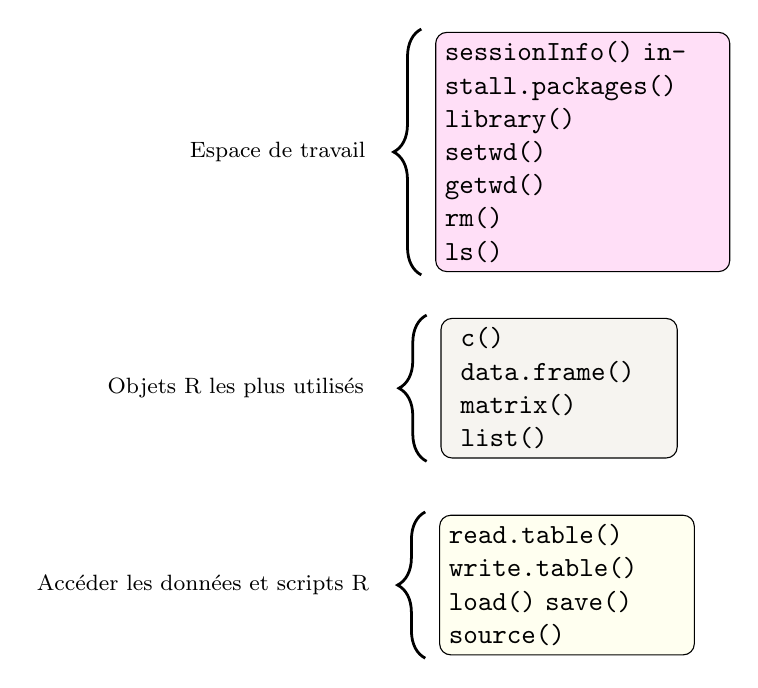
\begin{tikzpicture}
\node (expr) [startstop] {\code{sessionInfo()}
\code{install.packages()}
\code{library()}\textcolor{pinkish}{texxxx}
\code{setwd()}\textcolor{pinkish}{teccc}
\code{getwd()}\textcolor{pinkish}{teccc}
\code{rm()}\textcolor{pinkish}{tevvvvvvv}
\mbox{\code{ls()}\textcolor{pinkish}{tevvvvvvv}}  };
\node (fat) [startstop2, below of=expr, xshift=-.3cm, yshift=-2.0cm] {\code{c()}
\code{data.frame()}
\code{matrix()}
\code{list()}};
\node (script) [startstop3, below of=fat, xshift=.1cm, yshift=-1.5cm] {
\code{read.table()}
\code{write.table()}
\code{load()}
\code{save()}\textcolor{beige}{text}
\code{source()}};
\draw[decoration={brace,raise=5pt, amplitude=10pt},decorate,line width=1pt] 
  ([yshift=-1pt]expr.south west) -- ([yshift=1pt]expr.north west) node [black,midway,xshift=-2cm] 
{\footnotesize Espace de travail};
\draw[decoration={brace,raise=5pt,amplitude=10pt},decorate,line width=1pt] 
  ([yshift=-1pt]fat.south west) -- ([yshift=1pt]fat.north west) node [black,midway,xshift=-2.6cm] 
{\footnotesize Objets R les plus utilisés};
\draw[decoration={brace,raise=5pt,amplitude=10pt},decorate,line width=1pt] 
  ([yshift=-1pt]script.south west) -- ([yshift=1pt]script.north west) node [black,midway,xshift=-3cm] 
{\footnotesize Accéder les données et scripts R};
\end{tikzpicture}
%}
\end{frame}




\section{3. Graphiques}

\setbeamercolor{normal text}{fg=gray,bg=black}
\begin{frame}[plain]
\hspace*{-1.0cm}\parbox[t]{\textwidth}{
 \begin{center}
  \Huge{\textcolor{white}{3. Graphiques}}
 \end{center}
 }
\end{frame}

%\begin{comment}
\setbeamercolor{normal text}{fg=black,bg=background}
\begin{frame}[plain]
\hspace*{-1.0cm}\parbox[t]{\textwidth}{
\begin{block}{Objectifs du chapitre}
\begin{enumerate}
\item Comprendre la syntaxe de la fonction \code{plot}
\item Créer des \code{boxplot, histogram} et \code{density} plot
\item Comment sauvegarder des graphiques
\end{enumerate}
\end{block}
}
\end{frame}



\setbeamercolor{normal text}{fg=gray,bg=white}
\subsection{La fonction plot}

\begin{frame}
 \begin{center}
  \Huge{\textcolor{red}{La fonction \code{plot}}}
 \end{center}
\end{frame}



\begin{frame}[fragile]{Introduction aux graphiques en R}
\begin{itemize}
  \setlength\itemsep{2em}
  \item R offre une variété de graphiques remarquables 
  \item Pour avoir une petite idée des possibilités offertes, il suffit de taper la commande \code{demo(graphics)} 
\end{itemize}
\end{frame}


\begin{frame}[fragile]{La fonction \code{plot}}

\begin{itemize}
  \setlength\itemsep{2em}
\item La fonction \code{plot} peut prendre plusieurs arguments et types d'objets
\end{itemize}
\pause 
\begin{knitrout}
\definecolor{shadecolor}{rgb}{1, 1, 1}\color{fgcolor}\begin{kframe}
\begin{rcode}\label{unnamed-chunk-31}\begin{alltt}
\hlcom{# Plot des valeurs d'un vecteur contre leurs indices}
\hlcom{# équivalent à plot(mtcars[,"mpg"])}
\hlkwd{plot}\hlstd{(mtcars}\hlopt{$}\hlstd{mpg,} \hlkwc{xlab} \hlstd{=} \hlstr{"Index"}\hlstd{,} \hlkwc{ylab} \hlstd{=} \hlstr{"mpg"}\hlstd{,}
    \hlkwc{main} \hlstd{=} \hlstr{"Titre"}\hlstd{)}

\hlcom{# Graphique des couples (x, y)}
\hlkwd{plot}\hlstd{(mtcars}\hlopt{$}\hlstd{mpg, mtcars}\hlopt{$}\hlstd{disp,} \hlkwc{xlab} \hlstd{=} \hlstr{"mpg"}\hlstd{,}
\hlkwc{ylab} \hlstd{=} \hlstr{"disp"}\hlstd{,} \hlkwc{main} \hlstd{=} \hlstr{"mpg vs. disp"}\hlstd{)}
\end{alltt}
\end{rcode}\end{kframe}
\end{knitrout}

\end{frame}


\begin{frame}[fragile]{La fonction \code{plot}}

\begin{itemize}
  \setlength\itemsep{1.5em}
\item La fonction \code{plot} peut aussi prendre un objet du modèle linéaire comme argument
\pause \item Ceci est un exemple qui démontre pourquoi R est un langage orientée objet
\end{itemize}
\pause 
\begin{knitrout}
\definecolor{shadecolor}{rgb}{1, 1, 1}\color{fgcolor}\begin{kframe}
\begin{rcode}\label{unnamed-chunk-32}\begin{alltt}
\hlcom{# importer 'mtcars.RData'}
\hlkwd{load}\hlstd{(}\hlstr{"mtcars.RData"}\hlstd{)}

\hlcom{# Graphiques des 4 diagnostiques}
\hlcom{# du modèle linéaire}
\hlcom{# placer dans 2 rangés et 2 colonnes}
\hlkwd{par}\hlstd{(}\hlkwc{mfrow}\hlstd{=}\hlkwd{c}\hlstd{(}\hlnum{2}\hlstd{,}\hlnum{2}\hlstd{))}
\hlkwd{plot}\hlstd{(fit)}
\end{alltt}
\end{rcode}\end{kframe}
\end{knitrout}

\end{frame}


\subsection{\code{histogram} et \code{boxplot}}

\begin{frame}
 \begin{center}
  \Huge{\textcolor{red}{\code{histogram} et \code{boxplot}}}
 \end{center}
\end{frame}



\begin{frame}[fragile]{La fonction \code{histogram}}

\begin{itemize}
  \setlength\itemsep{1.5em}
  \item Utile pour voir la distribution des données
\item Pour les données continues et univariées
\end{itemize}
\pause 
\begin{knitrout}
\definecolor{shadecolor}{rgb}{1, 1, 1}\color{fgcolor}\begin{kframe}
\begin{rcode}\label{unnamed-chunk-33}\begin{alltt}
\hlcom{# la taille de 237 étudiants disponibles dans le jeu}
\hlcom{# de données 'survey' du library(MASS)}
\hlkwd{library}\hlstd{(MASS)}

\hlcom{# voir le nom des colonnes}
\hlkwd{names}\hlstd{(survey)}

\hlcom{# histogram de la taille et montrer la fréquence}
\hlcom{# de chaque barre}
\hlkwd{hist}\hlstd{(survey}\hlopt{$}\hlstd{Height,} \hlkwc{labels} \hlstd{=} \hlnum{TRUE}\hlstd{)}
\end{alltt}
\end{rcode}\end{kframe}
\end{knitrout}

\end{frame}





\begin{frame}[fragile]{La fonction \code{boxplot}}

\begin{itemize}
  \setlength\itemsep{2em}
\item Utile pour voir la différence d'une variable continue parmi plusieurs groupes
\end{itemize}
\pause 
\begin{knitrout}
\definecolor{shadecolor}{rgb}{1, 1, 1}\color{fgcolor}\begin{kframe}
\begin{rcode}\label{unnamed-chunk-34}\begin{alltt}
\hlcom{# visualiser la différence de taille entre les }
\hlcom{# hommes et les femmes dans le jeux}
\hlcom{# de données 'survey' du library(MASS)}

\hlkwd{boxplot}\hlstd{(survey}\hlopt{$}\hlstd{Height} \hlopt{~} \hlstd{survey}\hlopt{$}\hlstd{Sex,}
         \hlkwc{ylab} \hlstd{=} \hlstr{"Taille (cm)"}\hlstd{,}
         \hlkwc{col} \hlstd{=} \hlkwd{c}\hlstd{(}\hlstr{"lightpink"}\hlstd{,}\hlstr{"lightblue"}\hlstd{))}
\end{alltt}
\end{rcode}\end{kframe}
\end{knitrout}

\end{frame}


\begin{frame}[fragile]{Sauvegarder les graphiques}

\begin{itemize}
  \setlength\itemsep{2em}
\item 2 fonctions principales: \code{pdf()} et \code{png()}
\item l'argument de ces fonctions est le nom du fichier désiré
\end{itemize}
\pause 
\begin{knitrout}
\definecolor{shadecolor}{rgb}{1, 1, 1}\color{fgcolor}\begin{kframe}
\begin{rcode}\label{unnamed-chunk-35}\begin{alltt}
\hlcom{# enregistrer dans le répertoire de travail courant}
\hlkwd{pdf}\hlstd{(}\hlstr{"boxplot_survey.pdf"}\hlstd{)}
\hlkwd{boxplot}\hlstd{(survey}\hlopt{$}\hlstd{Height} \hlopt{~} \hlstd{survey}\hlopt{$}\hlstd{Sex,}
         \hlkwc{ylab} \hlstd{=} \hlstr{"Taille (cm)"}\hlstd{)}
\hlkwd{dev.off}\hlstd{()}
\end{alltt}
\end{rcode}\end{kframe}
\end{knitrout}

\end{frame}



\subsection{Sommaire}

\begin{frame}
 \begin{center}
  \Huge{\textcolor{red}{Sommaire}}
 \end{center}
\end{frame}




\begin{frame}{Sommaire des commandes de graphiques}
 %\hspace*{-1.9cm}\parbox[t]{\textwidth}{
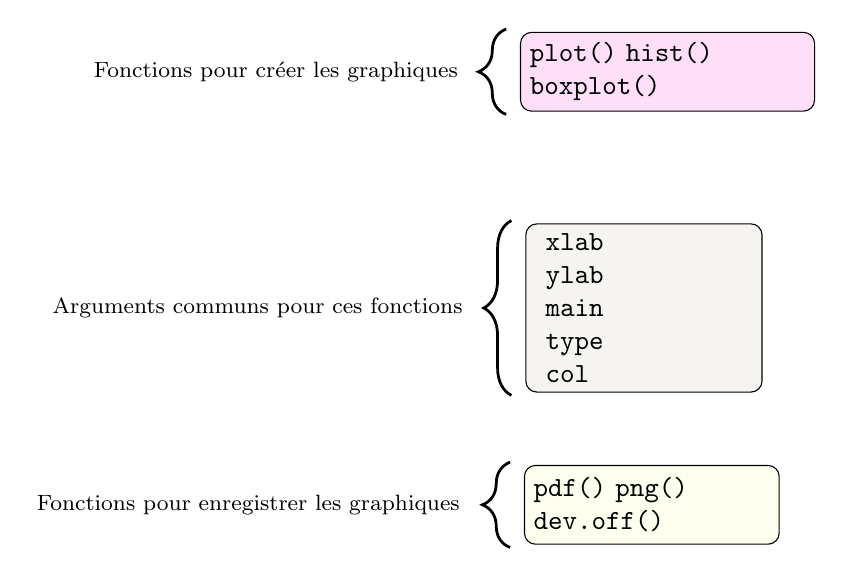
\begin{tikzpicture}
\node (expr) [startstop] {\code{plot()}
\code{hist()}\textcolor{pinkish}{texxxx}
\code{boxplot()}\textcolor{pinkish}{texxxx} };
\node (fat) [startstop2, below of=expr, xshift=-.3cm, yshift=-2.0cm] {\code{xlab}
\code{ylab}\textcolor{background}{textttt}
\code{main}\textcolor{background}{textttt}
\code{type}\textcolor{background}{textttt}
\code{col}\textcolor{background}{textttt}};
\node (script) [startstop3, below of=fat, xshift=.1cm, yshift=-1.5cm] {\code{pdf()}
\code{png()}\textcolor{beige}{textttt}
\code{dev.off()}\textcolor{beige}{textttt}}; 
\draw[decoration={brace,raise=5pt, amplitude=10pt},decorate,line width=1pt] 
  ([yshift=-1pt]expr.south west) -- ([yshift=1pt]expr.north west) node [black,midway,xshift=-3.1cm] 
{\footnotesize Fonctions pour créer les graphiques};
\draw[decoration={brace,raise=5pt,amplitude=10pt},decorate,line width=1pt] 
  ([yshift=-1pt]fat.south west) -- ([yshift=1pt]fat.north west) node [black,midway,xshift=-3.4cm] 
{\footnotesize Arguments communs pour ces fonctions};
\draw[decoration={brace,raise=5pt,amplitude=10pt},decorate,line width=1pt] 
  ([yshift=-1pt]script.south west) -- ([yshift=1pt]script.north west) node [black,midway,xshift=-3.5cm] 
{\footnotesize Fonctions pour enregistrer les graphiques};
\end{tikzpicture}
%}
\end{frame}





\section{4. Statistiques}

\setbeamercolor{normal text}{fg=gray,bg=black}
\begin{frame}[plain]
\hspace*{-1.0cm}\parbox[t]{\textwidth}{
 \begin{center}
  \Huge{\textcolor{white}{4. Statistiques}}
 \end{center}
 }
\end{frame}

\setbeamercolor{normal text}{fg=gray,bg=white}

\subsection{Moyenne, écart type}

\begin{frame}
 \begin{center}
  \Huge{\textcolor{red}{Moyenne, écart type}}
 \end{center}
\end{frame}



\begin{frame}[fragile]{Moyenne, variance, écart type, minimum, maximum}

\begin{itemize}
  \setlength\itemsep{2em}
\item fonctions principales: \code{mean(), var(), sd(), min(), max()}
\pause \item la fonction \code{summary()} est utile pour calculer quelques statistiques de bases pour un \textit{data frame}
\end{itemize}
\pause 
\begin{knitrout}
\definecolor{shadecolor}{rgb}{1, 1, 1}\color{fgcolor}\begin{kframe}
\begin{rcode}\label{unnamed-chunk-36}\begin{alltt}
\hlcom{# enregistrer dans le répertoire de travail courant}
\hlkwd{summary}\hlstd{(mtcars)}
\end{alltt}
\end{rcode}\end{kframe}
\end{knitrout}
\end{frame}




\begin{frame}[fragile]{La fonction \code{apply}}
\begin{itemize}
  \setlength\itemsep{1em}
\item Pour calculer des statistiques plus compliquées sur un \textit{data frame} (ou \textit{matrix}), on utilise la fonction \code{apply}
\pause \item La fonction \code{apply} sert à appliquer une fonction quelconque sur une partie d'un \textit{matrix} ou \textit{data frame}
\end{itemize}


\end{frame}



\begin{frame}[fragile]{La fonction \code{apply}}
\begin{itemize}
  \setlength\itemsep{1em}
\item La syntaxe de la fonction est la suivante:
\begin{center}
\code{apply(X, MARGIN, FUN)}
\end{center}
\item \code{X}: un matrix ou data frame
\item \code{MARGIN}: 1 si l'on veut faire des calculs sur les rangées, 2 sur les colonnes
\item \code{FUN}: est la fonction à appliquer
\end{itemize}
\pause 
\begin{knitrout}
\definecolor{shadecolor}{rgb}{1, 1, 1}\color{fgcolor}\begin{kframe}
\begin{rcode}\label{unnamed-chunk-37}\begin{alltt}
\hlcom{# variance par ligne}
\hlkwd{apply}\hlstd{(mtcars,} \hlnum{1}\hlstd{, var)}
\end{alltt}
\end{rcode}\end{kframe}
\end{knitrout}


\end{frame}









\begin{frame}[fragile]{La fonction \code{apply}}
\begin{knitrout}
\definecolor{shadecolor}{rgb}{1, 1, 1}\color{fgcolor}\begin{kframe}
\begin{rcode}\label{unnamed-chunk-38}\begin{alltt}
\hlcom{# variance par colonne}
\hlkwd{apply}\hlstd{(mtcars,} \hlnum{2}\hlstd{, var)}

\hlcom{# écart type par colonne}
\hlkwd{apply}\hlstd{(mtcars,} \hlnum{2}\hlstd{, sd)}

\hlcom{# minimum de chaque rangée}
\hlkwd{apply}\hlstd{(mtcars,} \hlnum{1}\hlstd{, min)}


\hlcom{# maximum de chaque rangée}
\hlkwd{apply}\hlstd{(mtcars,} \hlnum{1}\hlstd{, max)}
\end{alltt}
\end{rcode}\end{kframe}
\end{knitrout}


\end{frame}





\subsection{Test t et analyse de variance}

\begin{frame}
 \begin{center}
  \Huge{\textcolor{red}{Test t et analyse de variance}}
 \end{center}
\end{frame}



\begin{frame}[fragile]{Test t}

\begin{itemize}
  \setlength\itemsep{1.5em}
  \item la fonction pour faire un test t est \code{t.test()}
\end{itemize}
\pause 
\begin{knitrout}
\definecolor{shadecolor}{rgb}{1, 1, 1}\color{fgcolor}\begin{kframe}
\begin{rcode}\label{unnamed-chunk-39}\begin{alltt}
\hlcom{# la taille de 237 étudiants disponible dans le jeux}
\hlcom{# de données 'survey' du library(MASS)}
\hlcom{# est-ce qu'il y a une différence de taille entre}
\hlcom{# les hommes et les femmes?}

\hlkwd{t.test}\hlstd{(Height} \hlopt{~} \hlstd{Sex,} \hlkwc{data} \hlstd{= survey)}
\end{alltt}
\end{rcode}\end{kframe}
\end{knitrout}

\end{frame}







\begin{frame}[fragile]{Analyse de variance}

\begin{itemize}
  \setlength\itemsep{2em}
\item La fonction pour l'analyse de variance est \code{aov}
\pause \item Prenons un jeux de données disponible dans R: \code{InsectSprays}
\pause \item 6 insecticides ont été testés 12 fois en culture, la réponse observée étant le nombre d'insectes
\pause \item Le but c'est de voir s'il y a une différence importante entre les 6 insecticides par rapport à le nombre d'insectes
\end{itemize}


\end{frame}


\begin{frame}[fragile]{Analyse de variance}

\begin{knitrout}
\definecolor{shadecolor}{rgb}{1, 1, 1}\color{fgcolor}\begin{kframe}
\begin{rcode}\label{unnamed-chunk-40}\begin{alltt}
\hlcom{# boxplot pour voir la différence entre}
\hlcom{# les groupes}
\hlkwd{boxplot}\hlstd{(InsectSprays}\hlopt{$}\hlstd{count} \hlopt{~} \hlstd{InsectSprays}\hlopt{$}\hlstd{spray)}

\hlcom{# Les résultats ne sont pas affichés, ceux-ci sont }
\hlcom{# copiés dans un objet nommé aov.spray}
\hlstd{aov.spray} \hlkwb{<-} \hlkwd{aov}\hlstd{(count} \hlopt{~} \hlstd{spray,} \hlkwc{data} \hlstd{= InsectSprays)}

\hlcom{# sommaire des résultats}
\hlkwd{summary}\hlstd{(aov.spray)}
\end{alltt}
\end{rcode}\end{kframe}
\end{knitrout}

\end{frame}




\subsection{Modèles linéaires}

\begin{frame}
 \begin{center}
  \Huge{\textcolor{red}{Modèles linéaires}}
 \end{center}
\end{frame}


\begin{frame}[fragile]{Les formules}

\begin{itemize}
  \setlength\itemsep{1.5em}
  \item Les formules représentent un élément-clé des analyses statistiques avec R
  \pause \item La notation utilisée est la m\^{e}me pour (presque) toutes les fonctions
  \pause \item Une formule est typiquement de la forme 
  \begin{center}
  \code{y $\sim$ model}
  \end{center} 
  \pause \begin{enumerate}
  \item \code{y}: est la réponse analysée 
  \item \code{model}: est un ensemble de termes pour lesquels les paramètres sont estimés
  \end{enumerate}
  \pause \item Ces termes sont séparés par des symboles arithmétiques mais qui ont ici une signification
  particulière: \code{a+b}, \code{a*b}
 \end{itemize}
\end{frame}




\begin{frame}[fragile]{Modèles linéaires}

\begin{knitrout}
\definecolor{shadecolor}{rgb}{1, 1, 1}\color{fgcolor}\begin{kframe}
\begin{rcode}\label{unnamed-chunk-41}\begin{alltt}
\hlcom{# importer 'admit.txt'}
\hlstd{admit} \hlkwb{<-} \hlkwd{read.table}\hlstd{(}\hlstr{"admit.txt"}\hlstd{,} \hlkwc{header} \hlstd{=} \hlnum{TRUE}\hlstd{)}

\hlcom{# est-ce que gpa et rank sont reliés à gre}
\hlstd{fit} \hlkwb{<-} \hlkwd{lm}\hlstd{(gre} \hlopt{~} \hlstd{gpa}\hlopt{+}\hlstd{rank,} \hlkwc{data} \hlstd{= admit)}

\hlcom{# voir les résultats}
\hlkwd{summary}\hlstd{(fit)}
\end{alltt}
\end{rcode}\end{kframe}
\end{knitrout}

\end{frame}


\begin{frame}[fragile]{GLM}

\begin{knitrout}
\definecolor{shadecolor}{rgb}{1, 1, 1}\color{fgcolor}\begin{kframe}
\begin{rcode}\label{unnamed-chunk-42}\begin{alltt}
\hlcom{# régression logistique}
\hlstd{fit.glm} \hlkwb{<-} \hlkwd{glm}\hlstd{(admit} \hlopt{~} \hlstd{gre}\hlopt{+}\hlstd{gpa}\hlopt{+}\hlstd{rank,} \hlkwc{data} \hlstd{= admit,}
           \hlkwc{family} \hlstd{=} \hlkwd{binomial}\hlstd{(}\hlkwc{link} \hlstd{=} \hlstr{"logit"}\hlstd{))}

\hlcom{# voir les résultats}
\hlkwd{summary}\hlstd{(fit.glm)}
\end{alltt}
\end{rcode}\end{kframe}
\end{knitrout}

\end{frame}




\subsection{Sommaire}

\begin{frame}
 \begin{center}
  \Huge{\textcolor{red}{Sommaire}}
 \end{center}
\end{frame}




\begin{frame}{Sommaire des commandes de statistiques}
 %\hspace*{-1.9cm}\parbox[t]{\textwidth}{
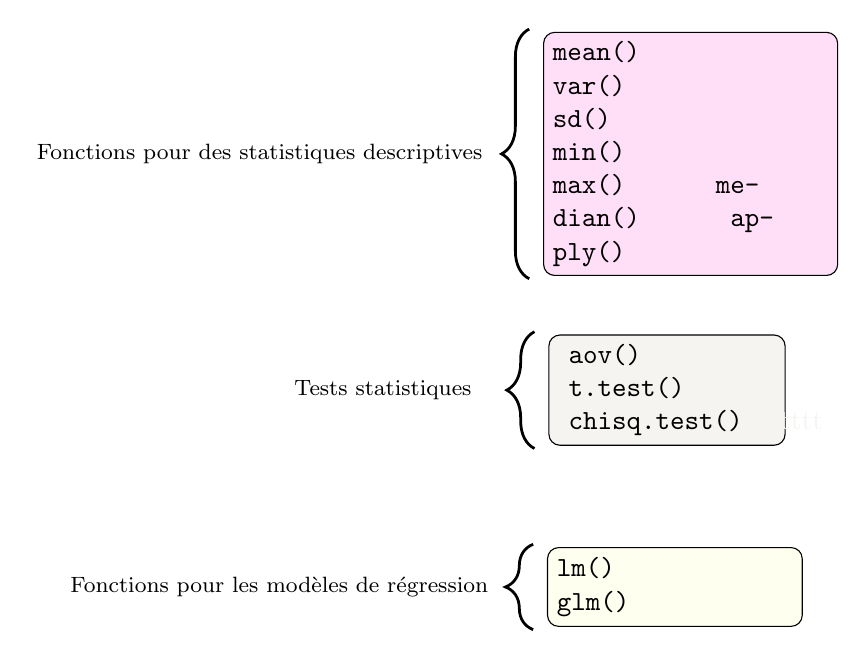
\begin{tikzpicture}
\node (expr) [startstop] {\code{mean()}
\code{var()}\textcolor{pinkish}{texxxxxx}
\code{sd()}\textcolor{pinkish}{texxxx} 
\code{min()}\textcolor{pinkish}{texxxx}
\code{max()}\textcolor{pinkish}{texxxx}
\code{median()}\textcolor{pinkish}{texxxx}
\code{apply()}\textcolor{pinkish}{texxxx}};
\node (fat) [startstop2, below of=expr, xshift=-.3cm, yshift=-2.0cm] {\code{aov()}
\code{t.test()}\textcolor{background}{textttt}
\code{chisq.test()}\textcolor{background}{textttt}};
\node (script) [startstop3, below of=fat, xshift=.1cm, yshift=-1.5cm] {\code{lm()}
\code{glm()}\textcolor{beige}{textdddttt}}; 
\draw[decoration={brace,raise=5pt, amplitude=10pt},decorate,line width=1pt] 
  ([yshift=-1pt]expr.south west) -- ([yshift=1pt]expr.north west) node [black,midway,xshift=-3.6cm] 
{\footnotesize Fonctions pour des statistiques descriptives};
\draw[decoration={brace,raise=5pt,amplitude=10pt},decorate,line width=1pt] 
  ([yshift=-1pt]fat.south west) -- ([yshift=1pt]fat.north west) node [black,midway,xshift=-2.1cm] 
{\footnotesize Tests statistiques};
\draw[decoration={brace,raise=5pt,amplitude=10pt},decorate,line width=1pt] 
  ([yshift=-1pt]script.south west) -- ([yshift=1pt]script.north west) node [black,midway,xshift=-3.4cm] 
{\footnotesize Fonctions pour les modèles de régression};
\end{tikzpicture}
%}
\end{frame}



\section{5. Rapports reproductibles}

\setbeamercolor{normal text}{fg=gray,bg=black}
\begin{frame}[plain]
\hspace*{-1.0cm}\parbox[t]{\textwidth}{
 \begin{center}
  \Huge{\textcolor{white}{5. Cr\'{e}er des rapports}}
 \end{center}
 }
\end{frame}

\setbeamercolor{normal text}{fg=gray,bg=white}
\subsection{Introduction}

\begin{frame}
 \begin{center}
  \Huge{\textcolor{red}{Introduction}}
 \end{center}
\end{frame}


\begin{frame}{Introduction}
\begin{itemize}
\item \href{http://rmarkdown.rstudio.com/}{http://rmarkdown.rstudio.com/}
\item \href{http://shiny.rstudio.com/gallery/}{http://shiny.rstudio.com/gallery/}
\end{itemize}
\end{frame}





\begin{frame}[fragile]{Session Information}
\begin{itemize}\raggedright
  \item R version 3.5.0 (2018-04-23), \verb|x86_64-w64-mingw32|
  \item Running under: \verb|Windows 10 x64 (build 17134)|
  \item Matrix products: default
  \item Base packages: base, datasets, graphics, grDevices, methods,
    stats, utils
  \item Other packages: data.table~1.11.0, dplyr~0.7.4,
    ggplot2~2.2.1, knitr~1.20, xtable~1.8-2
  \item Loaded via a namespace (and not attached): assertthat~0.2.0,
    bindr~0.1.1, bindrcpp~0.2.2, colorspace~1.3-2, compiler~3.5.0,
    evaluate~0.10.1, formatR~1.5, glue~1.2.0, grid~3.5.0,
    gtable~0.2.0, highr~0.6, lazyeval~0.2.1, magrittr~1.5,
    munsell~0.4.3, pillar~1.2.2, pkgconfig~2.0.1, plyr~1.8.4,
    R6~2.2.2, Rcpp~0.12.16, rlang~0.2.0, scales~0.5.0, stringi~1.1.7,
    stringr~1.3.0, tibble~1.4.2, tools~3.5.0
\end{itemize}


\end{frame}













\end{document}
